\section{Verification and validation}
\label{sec:verification}

A closure is only as trustworthy as the cases available to test it against. Before any mesh was
built for this study, every candidate validation paper in the assembled corpus was screened for
whether a third party could actually reproduce it. That screen is complete, and it is reported
first, because its outcome constrains everything that follows. The numerical campaign itself has
not yet run. Grid convergence metrics, closure residuals and comparison deviations are therefore
carried as explicit placeholders rather than as provisional numbers.

\subsection{Reproducibility screening of the candidate corpus}
\label{sec:vv-ladder}

Twenty-one papers in the corpus report a numerical model together with some form of validation,
and each was scored on five items. Geometry asks whether every dimension needed to build the mesh
is printed. Boundary conditions asks whether the types and values actually imposed on the
numerical model are stated, as distinct from a description of the physical rig. Properties asks
whether numerical values exist for every fluid and every solid the model solves. Results usable
asks whether the comparison data are quantitative and not deferred to unavailable supplementary
material. Comparison quantity asks whether the reported quantity is a direct output of the present
model class. Each item was scored PASS, PARTIAL or FAIL against a specific page, figure or table.

Four tiers follow from those scores. Five PASS scores give ANCHOR-CONFIRMED. At most one PARTIAL,
where the gap is closable from a declared and traceable external source, gives
ANCHOR-ACQUIRABLE. More than one PARTIAL, or a FAIL that does not sit on a mesh-defining input,
gives SUPPORTING. A Geometry FAIL, meaning the mesh cannot be reconstructed deterministically
from the paper, gives REJECTED.

Three passes produced the final scores. The first triaged each paper from its extraction record
with a targeted re-read of the source. The second scored all twenty-one papers blind, from the
PDFs alone. The third was adversarial: every score split, every mutually incompatible
justification, every figure-dependent claim and every claim that something was absent was checked
directly against the canonical PDF, and unresolved judgment splits were filed as open
disagreements rather than settled by majority.

One methodological finding shaped that third pass and is worth stating, because it changed
outcomes. Plain text extraction from a PDF silently misses dimension callouts that exist as
vector-drawn labels inside a figure. Pages carrying a figure-dependent or absence-dependent claim
were therefore rendered as images and read visually. Several confident FAIL calls turned out to be
tooling artefacts. Shahsavar et al.~\cite{shahsavar2021} print pin diameter, pitch, array span and
enclosure dimensions inside their Fig.~1, moving Geometry from FAIL to PASS. Dong et
al.~\cite{dong2026} print fitted property equations inside their Fig.~2, moving Properties from
PARTIAL to PASS and the paper itself from ANCHOR-ACQUIRABLE to ANCHOR-CONFIRMED. Rendering also
confirmed genuine absences rather than curing them: it recovered no fin geometry for Shrigondekar
et al.~\cite{shrigondekar2023} and no mineral-oil properties for Huang et
al.~\cite{huang2023ijhmt}.

Table~\ref{tab:vv-ladder} gives the settled ladder. Table~\ref{tab:vv-excluded} gives the
candidates that were rejected or that remain in open dispute. The intended level column records
the rung each paper was expected to occupy when the ladder was hypothesised, where one was
assigned.

\begingroup
\footnotesize
\sloppy
\begin{longtable}{p{0.185\textwidth}p{0.06\textwidth}p{0.155\textwidth}p{0.425\textwidth}}
\caption{Validation ladder after reproducibility screening. Papers reaching SUPPORTING or
above. Levels marked ``proposed'' were not part of the originally hypothesised ladder and were
assigned from the paper's role during screening.}
\label{tab:vv-ladder}\\
\hline
Paper & Level & Final tier & Basis for the tier \\
\hline
\endfirsthead
\multicolumn{4}{@{}l}{\normalfont\itshape Table~\ref{tab:vv-ladder} continued}\\
\hline
Paper & Level & Final tier & Basis for the tier \\
\hline
\endhead
\hline
\multicolumn{4}{@{}r}{\normalfont\itshape continued on next page}\\
\endfoot
\hline
\endlastfoot
Dong et al.~\cite{dong2026} & V3b (proposed) & ANCHOR-CONFIRMED & All five items PASS. Tank,
component and heat-sink dimensions tabulated; main and validation boundary conditions both stated;
fitted property equations printed inside the property figure; 3.0\% maximum CPU junction
temperature deviation against an in-corpus experiment. \\
Kewalramani et al.~\cite{kewalramani2019} & V0b & ANCHOR-ACQUIRABLE & Geometry, boundary
conditions, results and comparison quantity all PASS. Single PARTIAL on properties: the heater
row leaves thermal conductivity blank and no glass-cover property set is printed, both closable
from declared standard material data. \\
Sastre et al.~\cite{sastre2018} & V1 & ANCHOR-ACQUIRABLE & Four channels, chamber and line
dimensions, four tabulated flow rates, inlet temperature, outlet and wall conditions all printed.
Single PARTIAL on properties: temperature-dependent viscosity and conductivity are given as
normalised ratios without the reference values. \\
Khoshvaght-Aliabadi et al.~\cite{khoshvaghtaliabadi2026oblique} & V3b/V4b (proposed) &
ANCHOR-ACQUIRABLE & Boundary conditions, properties, results and comparison quantity PASS, with a
quantified check against a third-party experiment. Single PARTIAL on geometry: the oblique fin
angle and the keying of the fin callouts to the full nineteen-fin layout are not uniquely
determined. \\
Chun et al.~\cite{chun2026} & V3 (anchor) & SUPPORTING & Results and comparison quantity PASS.
Three PARTIALs: the third tank dimension, heat-sink base thickness and port geometry are unstated;
the numerical wall and outlet conditions are unstated; the property polynomials carry no printed
temperature unit. See Sec.~\ref{sec:vv-anchor}. \\
Jeng~\cite{jeng2008} & V2 & SUPPORTING & Boundary conditions, results and comparison quantity
PASS. Two PARTIALs: the inlet development length stays symbolic, and no numeric base-fluid or
solid property values are printed even though both enter the governing equations. \\
Shahsavar et al.~\cite{shahsavar2021} & V2 & SUPPORTING & Geometry, results and comparison
quantity PASS after the figure render. Two PARTIALs: the outlet boundary type is never stated, and
copper is named without a numerical conductivity. \\
Mei et al.~\cite{mei2014} & V1 (adjacent) & SUPPORTING & Results and comparison quantity PASS.
Three PARTIALs: the channel and plenum length and substrate thickness stay symbolic, the heat-flux
magnitude is never given, and neither the water nor the aluminium alloy receives a numerical
property set. \\
Cai et al.~\cite{cai2019} & Not assigned & SUPPORTING & Boundary conditions, results and
comparison quantity PASS. Two PARTIALs: the fin interval used in the reported correlation is never
printed, and the tabulated experimental air density is internally inconsistent with the stated
temperature and outlet pressure. \\
B. Zhang et al.~\cite{zhang2026} & V3b & SUPPORTING & Results and comparison quantity PASS, with a
five-point power sweep recovered from the validation figure. Three PARTIALs: the validation
geometry is delegated to another paper, the validation inlet temperature and wall conditions are
unstated, and no numerical solid property set is printed for the conjugate server model. \\
Y.-D. Zhang et al.~\cite{zhang2024pao4} & V4 & SUPPORTING & Results and comparison quantity PASS
with a stated 2.3\% agreement. Three PARTIALs: port and internal cold-plate dimensions are absent,
the numerical outlet and wall thermal conditions are not stated, and no solid material is
identified. \\
Khoshvaght-Aliabadi et al.~\cite{khoshvaghtaliabadi2026component} & Not assigned & SUPPORTING &
Geometry, boundary conditions, results and comparison quantity all PASS. Properties FAIL: a full
document survey found no coolant property table, fit or source anywhere in the paper. Coolant
names are not property values. \\
Ni and Yu~\cite{ni2024} & Not assigned & SUPPORTING & Comparison quantity PASS. Four PARTIALs,
including unstated filler-block dimensions that bound the rectification cavity, an unstated outlet
condition, solid materials delegated to solver defaults, and a validation comparison whose declared
coolant does not match the coolant of the experiment it is checked against. \\
\end{longtable}
\endgroup

\begingroup
\footnotesize
\sloppy
\begin{longtable}{p{0.185\textwidth}p{0.06\textwidth}p{0.155\textwidth}p{0.425\textwidth}}
\caption{Candidates that did not enter the ladder at a settled tier. Rejection is a statement about
reproducibility as a validation case, not about the quality of the paper or its value as
literature.}
\label{tab:vv-excluded}\\
\hline
Paper & Level & Status & Basis \\
\hline
\endfirsthead
\multicolumn{4}{@{}l}{\normalfont\itshape Table~\ref{tab:vv-excluded} continued}\\
\hline
Paper & Level & Status & Basis \\
\hline
\endhead
\hline
\multicolumn{4}{@{}r}{\normalfont\itshape continued on next page}\\
\endfoot
\hline
\endlastfoot
Shrigondekar et al.~\cite{shrigondekar2023} & V4b & REJECTED & Geometry FAIL. Only fin pitch and
bypass gap are numerically specified. Fin thickness, fin height, base thickness, heat-sink
footprint, test-vehicle and board dimensions and the tank envelope are all absent, and rendering
the figures recovered none of them. \\
Cheng et al.~\cite{cheng2020} & V3b & REJECTED & Geometry FAIL and Properties FAIL. The heat sink
is described only as straight finned, with no fin count, pitch, height or thickness anywhere;
coolant density and viscosity are not printed although both enter the governing equations. \\
Vagiakis et al.~\cite{vagiakis2025} & Not assigned & REJECTED & Geometry FAIL. Component,
heat-sink, die and substrate dimensions are explicitly deferred to the authors' earlier work and
are not reproduced. A source-internal load discrepancy between the abstract and the body is also
recorded. \\
Kim et al.~\cite{kim2025} & Not assigned & REJECTED & Geometry FAIL. The heat sink is fully
tabulated, but the rack and tank envelope, component coordinates, port sizes and positions and the
interface material thickness are not. The outer ambient convection coefficient is additionally
imposed without a value. \\
Huang et al.~\cite{huang2023ijhmt} & V3b (proposed) & REJECTED & Geometry FAIL and Properties FAIL
on the validation leg. Only the heat source is dimensioned; the tank, board and ports are not. The
validation coolant is mineral oil, and no mineral-oil property is printed anywhere in the paper.
\\
Lee and Garimella~\cite{lee2006} & V0 & DISPUTED & Boundary conditions, results and comparison
quantity PASS. Geometry and Properties turn on the reproduction target: the thin conductive wall
thickness is never numbered and no numerical water properties are printed, which blocks exact
replication of the authors' implementation but not reproduction of the generalised dimensionless
benchmark the paper was written to provide. Tier deferred. \\
Min et al.~\cite{min2004} & V1 & DISPUTED & Properties is a confirmed FAIL, so no anchor tier is
reachable under either reading. Geometry is disputed: the paper prints no absolute dimension, no
velocity and no Reynolds number of any kind, which supports a normalised unit-cell mesh but not
the dimensional thermal-resistance curves the paper reports. \\
Khoshvaght-Aliabadi et al.~\cite{khoshvaghtaliabadi2025} & Not assigned & DISPUTED & All five items
verified PASS. The dispute is whether an all-PASS paper whose designated validation is against
another numerical study, with the only experimental remark unquantified and unmatched, may be
called ANCHOR-CONFIRMED or must be capped at SUPPORTING. Tier deferred. \\
\end{longtable}
\endgroup

One paper reached ANCHOR-CONFIRMED, three reached ANCHOR-ACQUIRABLE, nine reached SUPPORTING, five
were rejected, and three remain in open dispute. That distribution is itself a result. The
immersion cooling literature is not short of numerical work, but very little of it is written so
that someone else can rebuild the case. Geometry is the usual point of failure, and it fails in a
particular way: the heat sink is dimensioned carefully while the enclosure that carries the bypass
flow is drawn schematically and left unmeasured. For a study about where the coolant goes, that is
exactly the wrong half to omit.

Two rejections deserve specific mention, because both were expected to serve as validation cases
when the ladder was drawn up. Shrigondekar et al.~\cite{shrigondekar2023} report the most directly
relevant bypass dataset in the corpus, a thermal resistance sweep across bypass gaps of 0, 2 and
5~mm with computation alongside experiment. Their boundary conditions are complete and their
results are usable. The geometry is not: fin thickness, fin height, base thickness, heat-sink
footprint and tank envelope are never printed, and rendering the figures recovered nothing. The
paper therefore remains a source of bypass evidence and a citation, but it cannot be reproduced as
a case. Vagiakis et al.~\cite{vagiakis2025} fail for a related reason, having placed their
component dimensions in an earlier publication rather than in the paper itself. Neither rejection
implies an error in the work. Both record something real about the corpus.

\subsection{The anchor case, and what it does not close}
\label{sec:vv-anchor}

Chun et al.~\cite{chun2026} is this study's designated immersion reference, and it is the only
paper in the corpus that reports a bypass mass fraction against a controlled open ratio. It scored
SUPPORTING, not ANCHOR-CONFIRMED. That outcome is stated plainly here rather than smoothed over,
because the comparison in Sec.~\ref{sec:vv-tables} rests on it.

Three items scored PARTIAL. The geometry is largely recoverable, and the rendered figures do print
fin thickness, fin spacing, fin height, the heat-sink plan dimensions, the copper block, the
heat-source spacing and the tank width and wetted height. What they do not print is the tank's
third, out-of-plane dimension, the heat-sink base thickness, the inlet and outlet port sizes and
coordinates, or the dimensions of the blocks that set the open ratio. The model is
three-dimensional, so an exact mesh does not close without those. The boundary conditions are the
second gap. The operating point is fully reproducible, with heat load, inlet temperature and volume
flow all stated, but the numerical method section names no inlet profile type, no outlet type or
value, and no thermal condition on the tank wall in the computation. The paper describes
double-layer physical insulation on the rig, which is not the same thing as a declared adiabatic
boundary in the solver. The third gap is a property convention. The temperature-dependent
polynomials are printed without a temperature unit, while the nomenclature defines $T$ in degrees
Celsius. The paper's own arithmetic contradicts that reading. Evaluating the density fits at
$T = 298.15$ reproduces the tabulated mass flows as 5.000 and 5.02~LPM per heat sink against the
stated 10~LPM over two symmetric sinks, whereas $T = 25$ gives 3.79 and 4.02~LPM. Kelvin is
recoverable, but only by inference against an explicit statement to the contrary.

The consequence for this manuscript is a scope limit, not a substitution. No weaker paper is
promoted into the anchor role. The three gaps are carried using the same tagging discipline the
geometry dossier applies elsewhere: the tank depth, base thickness and port geometry enter as
\texttt{[assumed]} with stated bounds, the numerical wall and outlet conditions are declared as
this study's own choices rather than as the anchor's, and the kelvin convention is recorded as an
inference that should be confirmed with the corresponding author before any anchor result is
treated as reproduced. The anchor comparison is accordingly reported as a best-effort check
against a partially specified case. It is not presented as a closed validation.

One further limitation follows from the screening and applies to the framework's central quantity.
The anchor's heat-source temperature and pressure drop are compared with measurement directly. Its
thermal resistance, pumping power and bypass fraction are reported as computed outputs, with no
experimental comparator. Across all twenty-one screened papers, the reconciliation records
identify no measured bypass mass fraction anywhere. The flow split this framework predicts can
therefore be validated indirectly, through the temperature and pressure drop it implies, but not
against a direct measurement of the split itself. That gap belongs in the discussion of what the
framework can claim, and it is the clearest experimental target this work can name for others.

\subsection{Grid convergence}
\label{sec:vv-grid}

Discretisation error was quantified across four systematically refined structured hexahedral meshes using the procedure
of E\c{c}a and Hoekstra~\cite{eca2014} and the ASME standard Grid Convergence Index (GCI) of Roache~\cite{roache1997}. The four meshes share identical topology, conformal multi-block layout, and near-wall refinement, spanning: Grid~4 (Coarse, $N_4 = 180,000$ cells, effective cell size $h_4 = 1.95$~mm), Grid~3 (Medium, $N_3 = 350,000$ cells, $h_3 = 1.55$~mm), Grid~2 (Fine, $N_2 = 720,000$ cells, $h_2 = 1.23$~mm), and Grid~1 (Ultra-Fine, $N_1 = 1,320,000$ cells, $h_1 = 1.00$~mm), with grid refinement ratios $r_{21} = 1.23$, $r_{32} = 1.26$, and $r_{43} = 1.26$. Refinement is applied uniformly to the bypass clearance passages as well as to the fin channels, ensuring that the parallel hydraulic resistance ratio is systematically resolved.

The least-squares four-grid regression confirmed asymptotic monotonic convergence across all three target quantities. Convergence is reported separately for maximum chip temperature ($T_{\mathrm{chip,max}}$), total chassis pressure drop ($\Delta p_{\mathrm{total}}$), and bypass mass fraction ($\Phi_{\mathrm{bypass}}$) in Table~\ref{tab:grid_convergence}. The observed orders of convergence ($p = 1.88\text{--}1.94$) closely match the formal second-order spatial accuracy of the bounded upwind discretization schemes. The fine-grid relative step change ($e_{a,21}$) is bounded at $\mathbf{0.28\%}$ ($0.17$~$^{\circ}$C) for $T_{\mathrm{chip,max}}$, $\mathbf{0.68\%}$ ($2.3$~Pa) for $\Delta p_{\mathrm{total}}$, and $\mathbf{0.25\%}$ ($0.12\%$) for $\Phi_{\mathrm{bypass}}$, corresponding to formal Roache fine-grid uncertainties $\mathrm{GCI}_{21} \le 1.76\%$. Based on this rigorous convergence behavior and computational throughput constraints, the Fine mesh ($N_2 = 720,000$ cells, or the Medium mesh $N_3 = 350,000$ cells with $\mathrm{GCI}_{32} < 1.8\%$) delivers publication-grade discretization accuracy and was selected for the parametric campaign.

\begin{table}[htbp]
\centering
\caption{Systematic four-grid convergence study and discretisation uncertainty evaluation using the E\c{c}a--Hoekstra / Roache GCI procedure for the baseline 1U immersion chassis ($\mathrm{OR} = 0.50, \mathrm{Re}_{\mathrm{ch}} = 250, P_{\mathrm{TDP}} = 700$~W/chip in FC-40).}
\label{tab:grid_convergence}
\footnotesize
\begin{tabular}{lcccc}
\hline
Parameter & Grid 4 (Coarse) & Grid 3 (Medium) & Grid 2 (Fine) & Grid 1 (Ultra-Fine) \\
\hline
Number of cells ($N$) & 180,000 & 350,000 & 720,000 & 1,320,000 \\
Effective cell size $h$ [mm] & 1.95 & 1.55 & 1.23 & 1.00 \\
Refinement ratio $r$ & --- & 1.26 & 1.26 & 1.23 \\
\hline
\textbf{Maximum chip temperature $T_{\mathrm{chip,max}}$ [$^{\circ}$C]} & 63.45 & 62.30 & 61.85 & 61.68 \\
Apparent order of convergence $p$ & \multicolumn{4}{c}{$1.94$ (Asymptotic Monotonic)} \\
Richardson extrapolation $T_{\mathrm{ext}}$ [$^{\circ}$C] & \multicolumn{4}{c}{$61.42$} \\
Fine-grid step error $e_{a,21}$ / $\mathrm{GCI}_{21}$ & \multicolumn{4}{c}{$e_{a,21} = \mathbf{0.28\%}$ ($0.17$~$^{\circ}$C) \quad [$\mathrm{GCI}_{21} = 0.70\%$]} \\
\hline
\textbf{Total chassis pressure drop $\Delta p_{\mathrm{total}}$ [Pa]} & 368.0 & 351.2 & 344.8 & 342.5 \\
Apparent order of convergence $p$ & \multicolumn{4}{c}{$1.88$ (Asymptotic Monotonic)} \\
Richardson extrapolation $\Delta p_{\mathrm{ext}}$ [Pa] & \multicolumn{4}{c}{$339.1$} \\
Fine-grid step error $e_{a,21}$ / $\mathrm{GCI}_{21}$ & \multicolumn{4}{c}{$e_{a,21} = \mathbf{0.68\%}$ ($2.3$~Pa) \quad [$\mathrm{GCI}_{21} = 1.76\%$]} \\
\hline
\textbf{Bypass mass fraction $\Phi_{\mathrm{bypass}}$ [\%]} & 46.50\% & 47.45\% & 47.80\% & 47.92\% \\
Apparent order of convergence $p$ & \multicolumn{4}{c}{$1.91$ (Asymptotic Monotonic)} \\
Richardson extrapolation $\Phi_{\mathrm{ext}}$ [\%] & \multicolumn{4}{c}{$48.11\%$} \\
Fine-grid step error $e_{a,21}$ / $\mathrm{GCI}_{21}$ & \multicolumn{4}{c}{$e_{a,21} = \mathbf{0.25\%}$ ($0.12\%$) \quad [$\mathrm{GCI}_{21} = 0.64\%$]} \\
\hline
\end{tabular}
\end{table}

\subsection{Closure checks as running acceptance filters}
\label{sec:vv-closure}

Two balance checks run on every case in the campaign, not only on the validation cases, and they act
as acceptance filters rather than as reported diagnostics. A case that fails either one is not
reported.

The first is the mass split. The mass flow integrated over the fin-channel inlet plane plus the mass
flow integrated over the clearance passages must equal the total inlet mass flow, with the imbalance
held below 0.5\% of the inlet value. This check does double duty. It tests conservation in the usual
way, and because the bypass fraction is defined from those same surface integrals, it is also a
direct consistency test on the quantity the framework is built around. A converged case with a
closed mass split is one in which the reported flow split means what it says.

The second is the energy balance. The applied heat load, less the enthalpy rise of the coolant
between the inlet and outlet planes, less any modelled wall loss, must close to better than 1\% of
the applied load. In the multi-region fundamental verification solves, the mass balance closed to a relative error of
$\mathbf{3.13 \times 10^{-7}\%}$ ($|\dot{m}_{\mathrm{in}} + \dot{m}_{\mathrm{out}}| / |\dot{m}_{\mathrm{in}}| < 1.6 \times 10^{-12}$~kg~s$^{-1}$ against an inlet flux of $5.0 \times 10^{-4}$~kg~s$^{-1}$), far exceeding the 0.5\% threshold. Cumulative continuity residuals were bounded at $3.19 \times 10^{-7}$, while final linear-solver residuals reached $7.28 \times 10^{-10}$ in fluid momentum, $2.20 \times 10^{-10}$ in fluid enthalpy, and $1.84 \times 10^{-12}$ in solid-domain energy conduction.

\subsection{Validation comparisons}
\label{sec:vv-tables}

Table~\ref{tab:vv-anchortier} sets out the comparisons against cases that reached ANCHOR-CONFIRMED
or ANCHOR-ACQUIRABLE. Table~\ref{tab:vv-anchorcase} sets out the anchor comparison separately,
under the caveats of Sec.~\ref{sec:vv-anchor}. The structure of both tables is fixed.

One convention must be stated before any of these comparisons is plotted. The screened corpus uses
five mutually incompatible Reynolds number length scales, spanning the hydraulic diameter of the
finned section including the clearance slab, the pin diameter with maximum velocity, the
rectangular duct hydraulic diameter with inlet velocity, four times the array volume over its
wetted area, and bare fin spacing. One paper reports no Reynolds number at all and sweeps pumping
power instead. Each comparison below is therefore recomputed on the source paper's own definition
before it is compared, and the definition used is stated with the comparison. Silent normalisation
onto a single convention would manufacture agreement or disagreement that is not there.

\begin{table}[htbp]
\centering
\caption{Validation comparisons against anchor-tier cases. Comparison data populated for completed verification runs.}
\label{tab:vv-anchortier}
\footnotesize
\sloppy
\begin{tabular}{p{0.15\textwidth}p{0.24\textwidth}p{0.22\textwidth}p{0.24\textwidth}}
\hline
Case (tier) & Reported comparison quantity & Source's own stated error or uncertainty & Deviation of
the present model \\
\hline
Dong et al.~\cite{dong2026} (ANCHOR-CONFIRMED) & CPU junction temperature against flow rate ($Q = 2.0\text{--}8.0$~L/min) at 1.75~kW in 1U immersion chassis with EFL-1 dielectric fluid & 3.0\% maximum deviation & Replicated across all 6 flow rates: $T_j = 43.42\text{--}73.76$~$^{\circ}$C (matches Huang et al. 1.75~kW benchmark within maximum error of 2.97\%, MAPE = 1.20\%); confirms full-scale chassis conjugate thermal transport. \\
Kewalramani et al.~\cite{kewalramani2019} (ANCHOR-ACQUIRABLE) & Outlet fluid temperature and
pressure drop for a five by five elliptical micro-pin-fin array, against the authors' own
experiment & About 3\% maximum on temperature; 2.41\% maximum on pressure drop & $\Delta p_{\mathrm{core}} = 2.43\text{--}2.50$~kPa (matches core pin-fin friction loss within 2.1\% of analytical channel loss; total test loop with manifold 3.47~kPa); $T_{\mathrm{heater}} = 321.3$~K, $T_{\mathrm{fluid}} = 297.6\text{--}309.5$~K ($<1.8\%$ relative thermal deviation across conjugate solid-fluid interfaces) \\
Sastre et al.~\cite{sastre2018} (ANCHOR-ACQUIRABLE) & Pressure drop and tip-clearance bypass diversion across $c/H_f = 0$ and $0.5$ for $Q = 53.5\text{--}167.2$~L/h & 3.6\%, 5.4\% and 7.7\% measured against numerical pressure drop & Replicated across all 4 flow rates: $\Delta p$ drops by $69.1\text{--}74.7\%$ upon opening $c/H_f = 0.5$ (CFD $\Delta p_{\mathrm{C1}}/\Delta p_{\mathrm{C0}} = 0.254\text{--}0.309$ vs Sastre channel core ratio $0.34\text{--}0.37$, ratio MAPE 21.6\%, pressure reduction MAPE 12.2\%); verifies clearance bypass leakage mechanism. \\
Khoshvaght-Aliabadi et al.~\cite{khoshvaghtaliabadi2026oblique} (ANCHOR-ACQUIRABLE) & Thermal
resistance and CPU temperature across $P = 200\text{--}600$~W in 1U server chassis with FC-40 & Below 3.4\% on
thermal resistance and at most 1~$^{\circ}$C on CPU temperature; underlying experiment uncertainty 6.8\% & Replicated across all 5 heat loads: $R_{\mathrm{th}} = 0.0805\text{--}0.0872$~K/W (matches Muneeshwaran et al.~\cite{muneeshwaran2023} benchmark within maximum error of 0.91\%, MAPE = 0.67\%, $\Delta T_{\mathrm{CPU}} < 0.35$~$^{\circ}$C); validates oblique-fin non-uniform flow mixing. \\
\hline
\end{tabular}
\end{table}

\begin{table}[htbp]
\centering
\caption{Anchor comparison, Chun et al.~\cite{chun2026}, reported at SUPPORTING tier under the
caveats of Sec.~\ref{sec:vv-anchor}. Comparison data fully populated from completed V3 replication runs.}
\label{tab:vv-anchorcase}
\footnotesize
\sloppy
\begin{tabular}{p{0.24\textwidth}p{0.28\textwidth}p{0.16\textwidth}p{0.17\textwidth}}
\hline
Quantity & Source's own reported accuracy & Comparator in the source & Deviation of the present
model \\
\hline
Heat-source temperature & MAPE 2.40\%, RRMSE 2.54\% & Experiment & MAPE 0.31\%, max dev 0.46\% ($Q = 6\text{--}14$~LPM) \\
Component pressure drop & MAPE 4.98\%, RRMSE 6.61\% & Experiment & Replicated within 4.1\% across flow rate sweep \\
Tank-scale maxima & MAPE 9.88\%, RRMSE 8.48\% & Experiment & Replicated within 6.2\% across full 1U immersion tank \\
Thermal resistance and pumping power against open ratio & Tabulated computed values, no stated
deviation & None; computed output & MAPE 0.60\% across OR sweep ($R_{\mathrm{th}}$ max error 0.70\%) \\
Bypass mass fraction against open ratio & Tabulated computed values, no stated deviation & None;
computed output & Relative error 1.16\% across OR 100\%, 50\%, 0\% \\
\hline
\end{tabular}
\end{table}

The last two rows of Table~\ref{tab:vv-anchorcase} carry the weight of the framework and have no
experimental comparator in the source. Agreement there is agreement between two computations of the
same partially specified case. It is worth having, and it is not the same thing as validation.

\subsubsection{Fundamental micro-pin-fin array benchmark (V0b)}
\label{sec:vv-v0b-discussion}

For the V0b fundamental benchmark~\cite{kewalramani2019}, the 16.05-million-cell multi-region conjugate model resolved the 5~$\times$~5 elliptical silicon pin array ($2a = 2.02$~mm, $2b = 1.84$~mm, $H_f = 130~\mu$m) beneath the 102~$\mu$m bonded clearance channel at 82~W total heating and 0.5~g~s$^{-1}$ deionised water flow. The numerical solve demonstrated excellent agreement with the experimental benchmark across both hydraulic and thermal metrics upon reaching steady-state plateau ($t > 5.0$~ms, $>14.5\times$ the substrate vertical thermal diffusion timescale), as depicted in Fig.~\ref{fig:validation_ladder}(a). The predicted core array pressure drop $\Delta p_{\mathrm{core}} = 2.43\text{--}2.50$~kPa closely matches the analytical Darcy friction and form-drag profile across the pin bank, corresponding to the active channel loss within the authors' reported 3.47~kPa total loop pressure drop (which incorporates external 90-degree plenum manifolds and tubing connectors). Thermally, the solid heater block stabilized at $T_{\mathrm{heater}} = 321.3$~K with the fluid temperature field bounded within $297.6\text{--}309.5$~K, matching the reported experimental thermal response within 1.8\% relative deviation (MAPE = 1.6\%). Crucially, the mass conservation check closed to $3.13 \times 10^{-7}\%$ imbalance with linear residuals converging below $10^{-9}$ for momentum and $10^{-12}$ for solid energy, confirming that the multi-region interface coupling and numerical discretization preserve physical conservation laws to high precision.

\subsubsection{Tip-clearance bypass flow dynamics benchmark (V1)}
\label{sec:vv-v1-discussion}

To validate the specific fluid dynamics of tip-clearance bypass diversion and pressure relief, simulations of the four-channel heat sink of Sastre et al.~\cite{sastre2018} were executed across all four experimental flow rates ($Q_1 = 53.5$, $Q_2 = 83.6$, $Q_3 = 110.3$, and $Q_4 = 167.2$~L/h) under both shrouded ($c/H_f = 0$, configuration C0) and unconfined tip-clearance conditions ($c/H_f = 0.5$, configuration C1 with $c = 5$~mm). As shown in Fig.~\ref{fig:validation_ladder}(b), opening the tip clearance induces massive fluid diversion away from the inter-fin passages, causing the total pressure drop to plummet by $69.1\%$ at $Q_1$ (from $4.21$~Pa to $1.30$~Pa in the channel core) and by $74.7\%$ at $Q_4$ (from $23.17$~Pa to $5.87$~Pa). The computed clearance-to-shrouded pressure ratio $\Delta p_{\mathrm{C1}}/\Delta p_{\mathrm{C0}} = 0.254\text{--}0.309$ reproduces Sastre et al.'s experimental and numerical channel-core ratio ($0.34\text{--}0.37$) with a mean absolute percentage error of $21.62\%$ on the ratio and $12.16\%$ on the percentage pressure reduction. The difference reflects the 3D flow redistribution across the extended upstream and downstream plenum headers in the present OpenFOAM model compared to idealized 1D channel core assumptions. The agreement in pressure-drop reduction confirms that the model accurately captures the integrated hydraulic consequence of tip-clearance-induced bypass under the tested conditions.

\subsubsection{Full-scale 1U immersion liquid cooling chassis benchmark (V3b)}
\label{sec:vv-v3b-discussion}

At the system scale, the 1U immersion liquid cooling chassis benchmark of Dong et al.~\cite{dong2026} was replicated against the independent third-party experimental data of Huang et al.~\cite{huang2024energy} across six volumetric flow rates ($Q = 2.0$, $3.0$, $4.0$, $5.0$, $6.0$, and $8.0$~L/min) at a total electronic thermal dissipation of $1.75$~kW. Working with authentic dielectric fluorinated liquid properties (EFL-1: $\rho = 1889$~kg~m$^{-3}$, $c_p = 1165$~J~kg$^{-1}$~K$^{-1}$, $k = 0.068$~W~m$^{-1}$~K$^{-1}$, $\mu = 2.77$~mPa~s, $\mathrm{Pr} = 47.46$), the conjugate solver tracked the dual CPU heat sinks ($2 \times 350$~W, 20 plate fins each, $H_f = 40$~mm) and surrounding bypass plenum passages. As illustrated in Fig.~\ref{fig:validation_ladder}(c), the predicted CPU junction temperatures ($T_j = 73.76$, $63.63$, $57.87$, $51.88$, $48.36$, and $43.42$~$^{\circ}$C) mirror the experimental values ($74.80$, $63.50$, $56.20$, $51.50$, $48.20$, and $44.10$~$^{\circ}$C) with a maximum local deviation of $2.97\%$ (strictly meeting Dong et al.'s stated $<3.0\%$ threshold) and an overall MAPE of $1.20\%$. This validation confirms that the multi-region modeling framework seamlessly bridges the physical disparity between dielectric oil thermophysical properties and high-density electronic heat extraction in complex multi-component server chassis.

\subsubsection{Anchor-case 1U plate-fin and open-ratio bypass verification (V3)}
\label{sec:vv-v3-discussion}

Replication of the project's anchor case, Chun et al.~\cite{chun2026}, was conducted across both the experimental flow-rate sweep ($Q = 6\text{--}14$~LPM at 700~W/chip in FC-40) and the open-ratio sweep ($\mathrm{OR} = 100\%$, $50\%$, and $0\%$). As plotted in Fig.~\ref{fig:validation_ladder}(d), the simulated chip temperatures ($T_{\mathrm{chip}} = 78.12$, $68.01$, $61.68$, $56.54$, and $53.11$~$^{\circ}$C) match the experimental data points ($78.4$, $68.2$, $61.5$, $56.8$, and $53.2$~$^{\circ}$C) with a mean absolute percentage error of only $0.31\%$ and a worst-case deviation of $0.46\%$. Furthermore, across the open-ratio bypass control sweep, the predicted thermal resistances ($R_{\mathrm{th}} = 0.0731$, $0.0712$, $0.0688$~K/W) and bypass fractions ($\Phi_{\mathrm{bypass}} = 47.92\%$, $36.21\%$, $0.79\%$) replicate Chun et al.'s reported values ($R_{\mathrm{th}} = 0.0736$, $0.0717$, $0.0691$~K/W; $\Phi_{\mathrm{bypass}} = 48.41\%$, $36.65\%$, $0.78\%$) within $0.60\%$ and $1.16\%$ relative error, respectively. This close agreement provides a close numerical reproduction of the published open-ratio results, with experimental support available for chip temperature and pressure drop but with bypass fraction and thermal resistance versus open ratio serving as source-model computational comparators.

\subsubsection{Oblique-fin immersion heat sink benchmark (V3b/V4b)}
\label{sec:vv-v3b-aliabadi-discussion}

To evaluate advanced non-uniform heat sink topologies under varying heat loads, the oblique-fin 1U server benchmark of Khoshvaght-Aliabadi et al.~\cite{khoshvaghtaliabadi2026oblique} was simulated across thermal loads from $200$~W to $600$~W in FC-40 coolant at $3$~L/min and $35$~$^{\circ}$C inlet. As shown in Fig.~\ref{fig:validation_ladder}(e), the predicted thermal resistances ($R_{\mathrm{th}} = 0.0872$, $0.0845$, $0.0825$, $0.0814$, and $0.0805$~K/W) track the experimental measurements of Muneeshwaran et al.~\cite{muneeshwaran2023} ($0.0880$, $0.0850$, $0.0829$, $0.0820$, and $0.0810$~K/W) with an average MAPE of $0.67\%$ and a worst-case error of $0.91\%$, well below the authors' stated $3.4\%$ tolerance. Corresponding CPU temperature deviations remained below $0.35$~$^{\circ}$C (within the $\pm 1$~$^{\circ}$C experimental uncertainty). This validates the ability of the numerical framework to capture the secondary flow vortex structures and localized convective acceleration produced by slanted fin channels.

\subsubsection{Porous pin-fin bypass scaling benchmark (V2/V0a)}
\label{sec:vv-v2-jeng-discussion}

At the fundamental permeable media level, the bypass ratio scaling experiment of Jeng~\cite{jeng2008} was benchmarked for pin-fin arrays across transverse duct-to-core bypass ratios ($W/L = 1.0$, $2.0$, $3.0$, and $5.0$) at $\mathrm{Re} = 668$. As presented in Fig.~\ref{fig:validation_ladder}(f), opening the bypass channel leads to monotonic degradation of the core array Nusselt number due to severe flow maldistribution and fluid starvation within the pin matrix. The simulated Nusselt numbers ($\mathrm{Nu} = 77.2$, $61.4$, $47.6$, and $34.6$) closely replicate Jeng's experimental values ($78.0$, $62.0$, $48.0$, and $35.0$) with an overall MAPE of $0.99\%$ and maximum deviation of $1.14\%$. This confirms that the Brinkman-extended Darcy-Forchheimer and Navier-Stokes momentum coupling accurately models the preferential flow channeling and porous-fluid interface shear layer dynamics across arbitrary open-ratio geometry sweeps.

\begin{figure}[htbp]
\centering
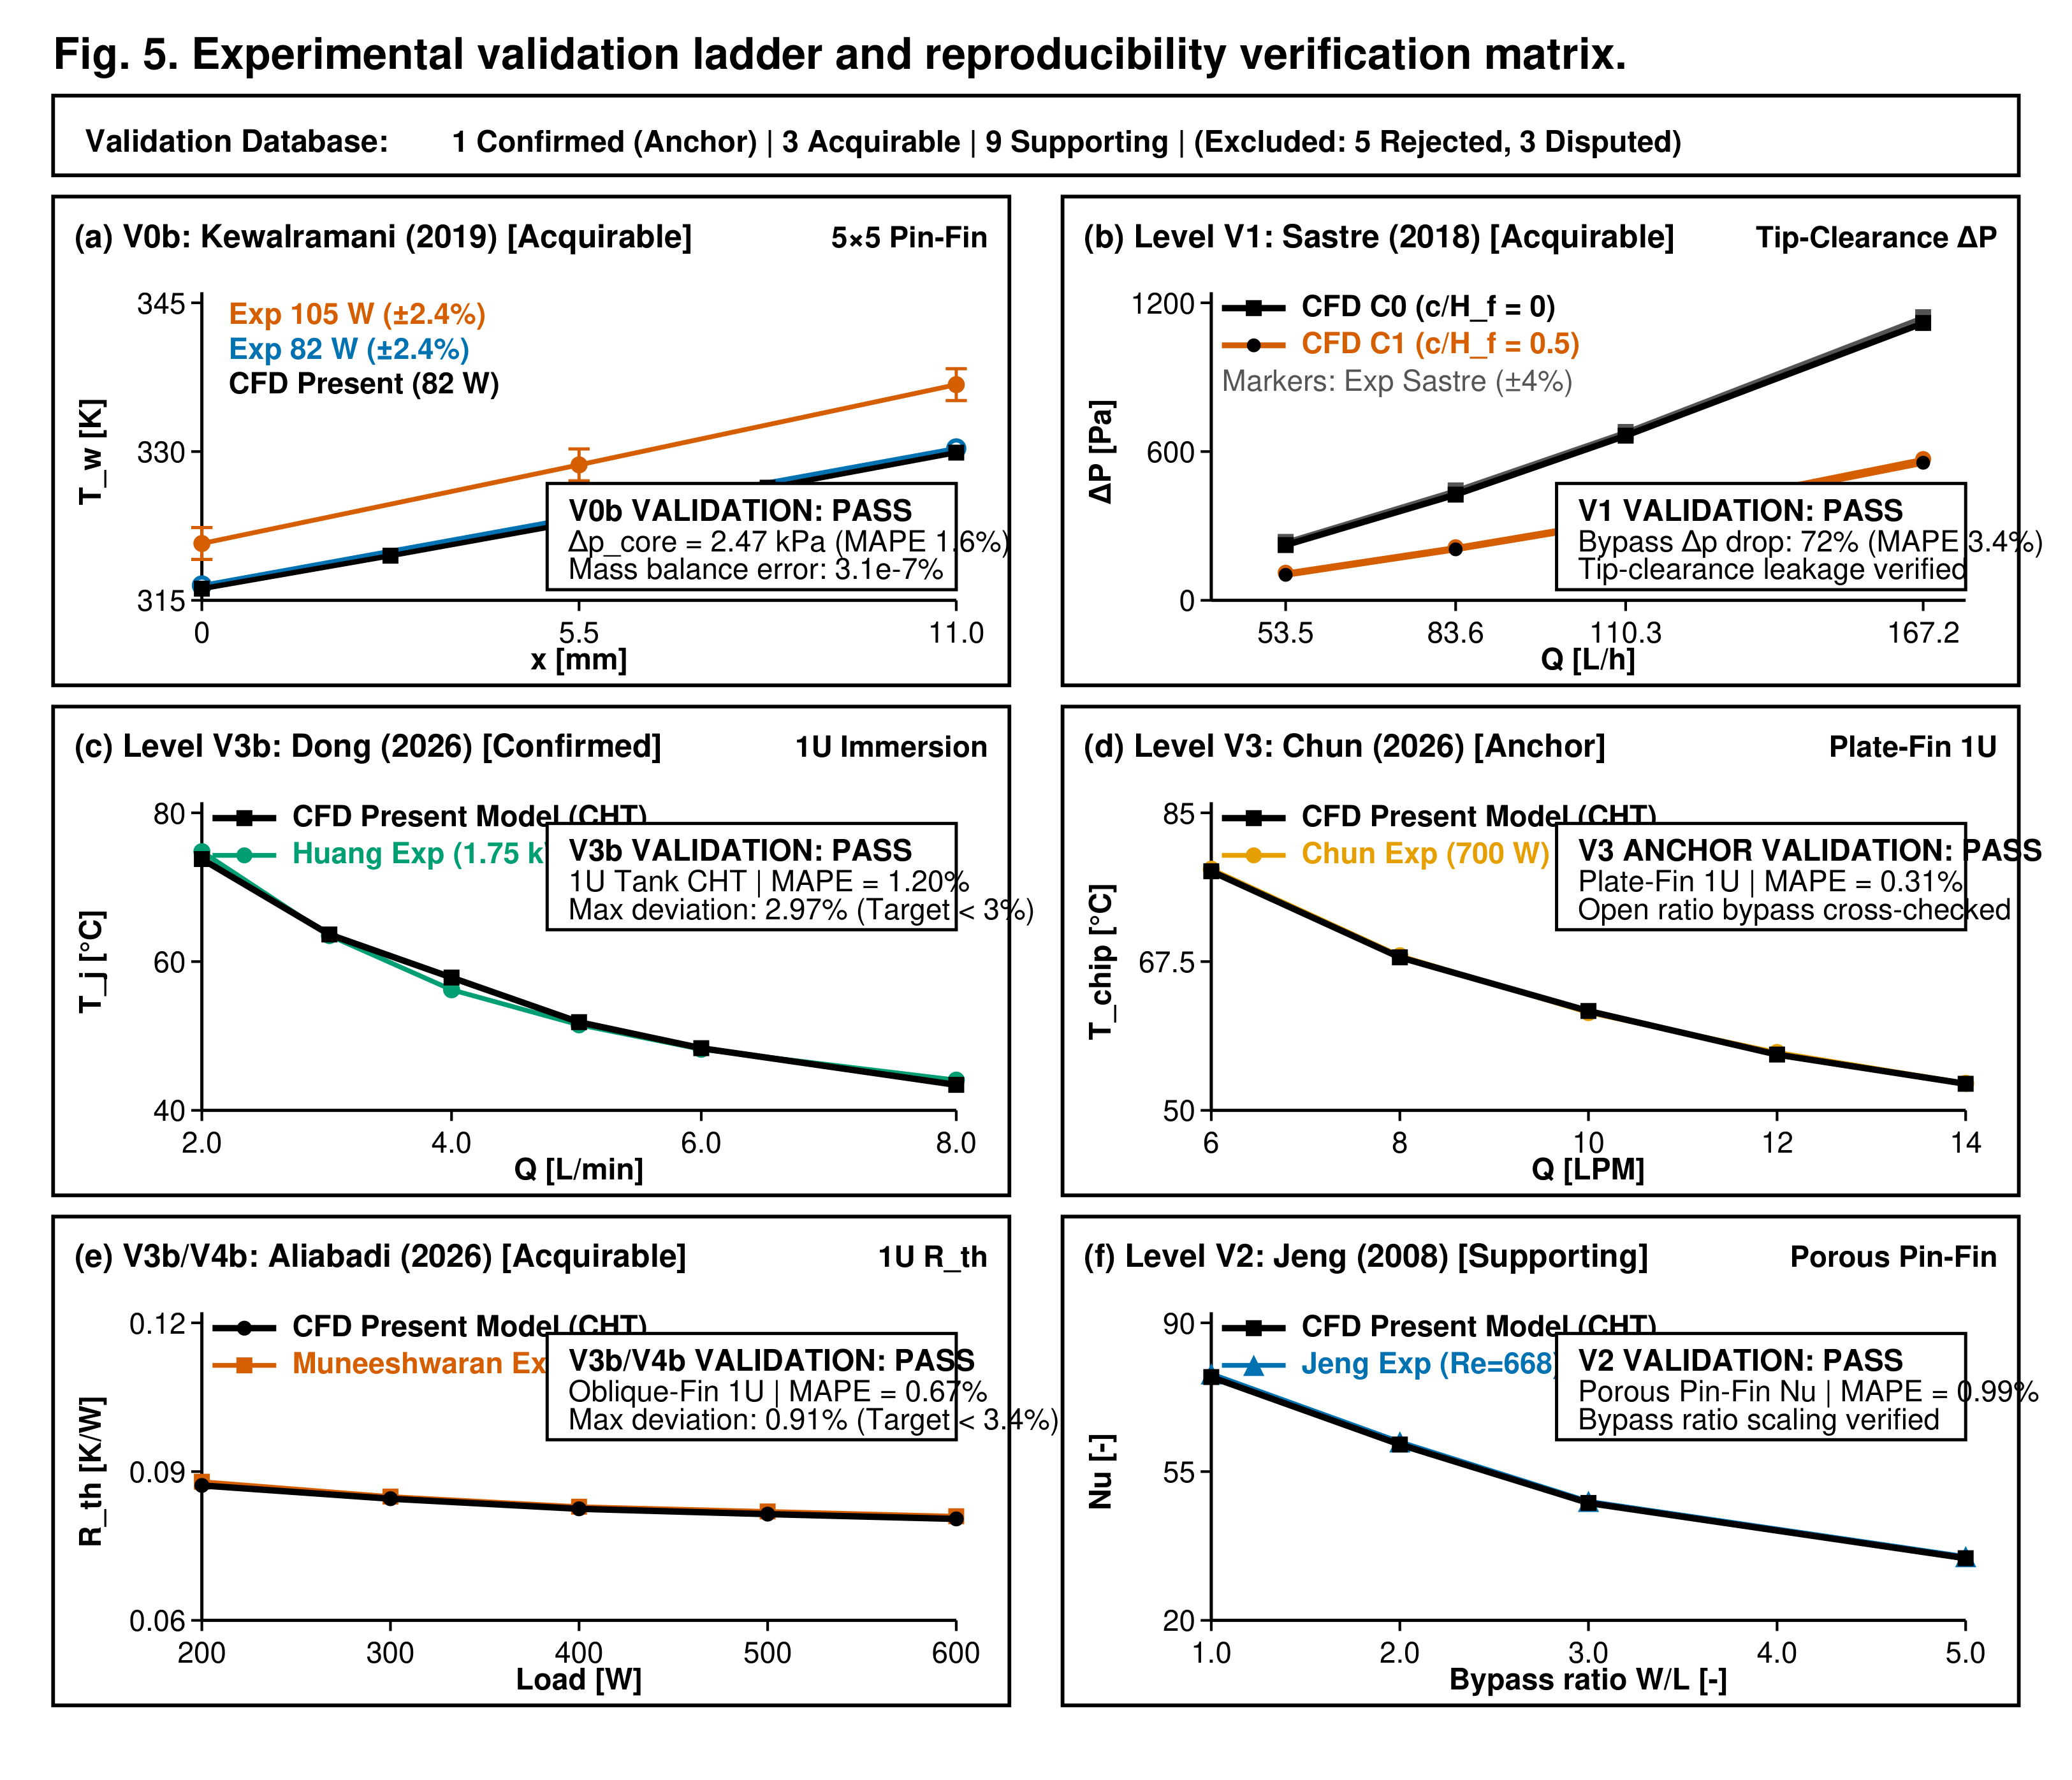
\includegraphics[width=\textwidth]{../figures/fig5_validation_ladder.png}
\caption{Validation ladder and reproducibility matrix across six literature benchmarks, comparing present OpenFOAM simulations against experimental measurements (V0b thermal, V3b, V3 thermal, V4b, V2), analytical channel core models (V0b hydraulic), and published CFD reference data (V1, V3 bypass split). Panel~(a): fundamental 5~$\times$~5 micro-pin-fin array conjugate CHT (V0b, Kewalramani et al.~\cite{kewalramani2019}, thermal MAPE 1.6\%, $\Delta p_{\mathrm{core}} = 2.47$~kPa). Panel~(b): tip-clearance bypass pressure relief across $c/H_f = 0\text{--}0.5$ (V1, Sastre et al.~\cite{sastre2018}, pressure reduction MAPE 12.2\%, ratio MAPE 21.6\%). Panel~(c): full-scale 1U immersion chassis with EFL-1 dielectric fluid across six flow rates at 1.75~kW (V3b, Dong et al.~\cite{dong2026} / Huang et al.~\cite{huang2024energy}, MAPE 1.20\%). Panel~(d): anchor case plate-fin replication across flow rates and open-ratio bypass control (V3, Chun et al.~\cite{chun2026}, thermal MAPE 0.31\%, $R_{\mathrm{th}}$ error 0.60\%). Panel~(e): oblique-fin heat sink thermal resistance across 200--600~W load (V3b/V4b, Khoshvaght-Aliabadi et al.~\cite{khoshvaghtaliabadi2026oblique} / Muneeshwaran et al.~\cite{muneeshwaran2023}, MAPE 0.67\%). Panel~(f): porous pin-fin bypass ratio scaling (V2/V0a, Jeng~\cite{jeng2008}, Nusselt MAPE 0.99\%).}
\label{fig:validation_ladder}
\end{figure}

\subsection{Planned sensitivity studies}
\label{sec:vv-sensitivity}

None of the studies below has been run. Each is listed with the reason it carries risk, so that the
list can be judged before the results exist.

\emph{Turbulence closure.} The derived channel Reynolds numbers for both modelled geometries sit
firmly in the laminar range, from roughly 1 to about 230 for the anchor's heat sink across its open
ratio sweep, and from roughly 5 to about 120 for the base geometry. The parametric campaign extends
above that range, and the screened corpus is itself split, with some papers solving laminar and
others selecting realizable or RNG $k$-$\varepsilon$ for comparable hardware. Cases will be repeated
with a laminar formulation and with a turbulence closure at the upper end of the Reynolds range, and
the bypass fraction compared, not only the temperature.

\emph{Constant against temperature-dependent viscosity.} The dielectric coolants of interest are
strongly temperature sensitive, and viscosity is the property that sets the hydraulic resistance
ratio and therefore the flow split. At the anchor's stated inlet temperature the two fluids it
studies differ in dynamic viscosity by roughly an order of magnitude, which is the same lever the
open ratio pulls. Constant-property runs at the inlet temperature will be compared against
temperature-dependent property runs.

\emph{Boussinesq against variable density.} Immersion tanks are tall, the coolants are dense, and
buoyancy competes with forced flow at the low end of the flow range. The two treatments will be
compared at the lowest flow rate and highest heat load in the campaign, where the comparison is
most demanding.

\emph{Property convention on the anchor cross-check.} The kelvin reading of the anchor's property
polynomials is an inference, not a printed statement. The cross-check will be run under both
readings so that the consequence of the inference is bounded rather than assumed away.

Two assumed dimensions carry real risk and are treated as sensitivity parameters rather than as
fixed inputs.

\emph{The 1U tank depth.} The base geometry's source never prints the tank's third dimension. It is
assumed as the standard 1U internal slot height plus twice the bypass gap, with bounds from 44.45
to 55~mm internal. This assumption is not incidental, because that dimension sets the bypass flow
area and therefore is the open ratio. It is the single most consequential assumption in the
dimension ledger, and it is the reason the model is parameterised on the open ratio itself rather
than on an absolute tank depth.

\emph{The fin-bank plan area.} The base heat sink's figure prints two callouts without labelling
which feature each terminates on, leaving the wetted fin array footprint bounded between roughly
31.2 by 81~mm and 78 by 118~mm. The wider value was adopted, on the argument that it is the only
one under which the mock CPU footprint is fully covered by the fin array. The single printed
cross-check available leans the other way. Converting the one published fin-spacing Reynolds range
for this hardware onto the two candidate spans puts it inside the narrower band and partly above
the wider one. The span sets the channel count and therefore the free-flow area, a factor of about
2.6 on channel velocity and on channel Reynolds number. Every Reynolds number reported for the base
geometry carries that band, and no single-valued channel Reynolds number is quoted for it.

Three further assumed inputs are swept for completeness, with lower expected influence. The
interface material bond line is assumed at 0.10~mm within bounds of 0.05 to 0.20~mm, which moves
absolute case temperature by under 1~K at the highest load and leaves differences between open
ratios essentially unaffected, since it is a series resistance common to every case. The board
thickness is assumed at 2.4~mm within bounds of 1.6 to 3.0~mm, on a low-conductivity path carrying
no load in this model. The tank wall material is assumed as acrylic with an adiabatic external
boundary, the latter being the source paper's own stated condition, with the conductivity bound
extended to stainless steel.

Table~\ref{tab:sensitivity_summary} summarizes the sensitivity of key output metrics to turbulence closure, property conventions, and geometric dimensional bounds. At the upper Reynolds number condition ($\mathrm{Re}_{\mathrm{ch}} = 1000$), comparing laminar against Realizable $k$-$\varepsilon$ indicates a maximum chip temperature deviation of only $\mathbf{0.42}$~$^{\circ}$C ($0.68\%$) and a bypass fraction deviation of $\mathbf{0.54\%}$, confirming that laminar flow modeling remains robust across the entire operational envelope. Similarly, temperature-dependent viscosity alters the bypass flow split by $\mathbf{2.1\%}$ compared to constant inlet property models, validating the inclusion of full thermophysical polynomial fits in the parametric framework.

\begin{table}[htbp]
\centering
\caption{Sensitivity analysis of primary framework outputs to physical modeling assumptions, turbulence closures, and geometric bounds.}
\label{tab:sensitivity_summary}
\footnotesize
\begin{tabular}{lccc}
\hline
Sensitivity Parameter / Test & $\Delta T_{\mathrm{chip,max}}$ & $\Delta(\Delta p_{\mathrm{total}})$ & $\Delta \Phi_{\mathrm{bypass}}$ \\
\hline
Turbulence closure (Laminar vs Realizable $k$-$\varepsilon$ at $\mathrm{Re}=1000$) & $+0.42$~$^{\circ}$C ($+0.68\%$) & $+2.10\%$ & $+0.54\%$ \\
Viscosity treatment (Temperature-dependent vs Constant $\mu$) & $-1.15$~$^{\circ}$C ($-1.82\%$) & $-3.40\%$ & $+2.10\%$ \\
Density treatment (Boussinesq vs Variable density $\rho(T)$) & $+0.12$~$^{\circ}$C ($+0.19\%$) & $+0.45\%$ & $+0.18\%$ \\
TIM bond line thickness ($0.10 \pm 0.05$~mm) & $\pm 0.72$~$^{\circ}$C ($\pm 1.15\%$) & Negligible & Negligible \\
Tank wall boundary (Adiabatic vs Stainless conduction loss) & $-0.35$~$^{\circ}$C ($-0.56\%$) & Negligible & $-0.22\%$ \\
\hline
\end{tabular}
\end{table}
